\documentclass[10pt]{article}
\usepackage{graphicx} % Required for inserting images
\usepackage{geometry}
\usepackage[english,spanish]{babel}
\usepackage{blindtext}
\usepackage{lipsum}
\usepackage{parskip}
\usepackage{setspace}
\usepackage{caption}
\usepackage{multicol}
\usepackage{hyperref}
\usepackage{float}
\usepackage{changepage}
\usepackage{longtable}
\usepackage{multirow}
\usepackage{ragged2e}
\usepackage[style=apa,backend=biber]{biblatex}
\addbibresource{referencias.bib}
\usepackage{tabularx}
\usepackage{array}
\usepackage[utf8]{inputenc}
\usepackage[T1]{fontenc}
\usepackage[spanish]{babel}
\usepackage{amsmath}
\usepackage{booktabs}

\usepackage{parskip}

\usepackage{tikz}

\usetikzlibrary{shapes, arrows}
\usetikzlibrary{shapes.geometric}
\usetikzlibrary{positioning}
\usetikzlibrary{positioning, arrows.meta}
\usetikzlibrary{shapes, arrows.meta}

\tikzstyle{block} = [rectangle, draw, fill=blue!20, text width=6em, text centered, rounded corners, minimum height=3em]
\tikzstyle{line} = [draw, -latex']
\tikzstyle{cloud} = [draw, ellipse, fill=red!20, node distance=3cm, minimum height=2em]

\usepackage{schemata}
\usetikzlibrary{mindmap}

\usetikzlibrary{fit,positioning}

\geometry{
    top=2.5cm,
    left=2.8cm,
    right=2.8cm,
    bottom=2.44cm
}

\tikzset{
every picture/.append style={
  execute at begin picture={\deactivatequoting},
  execute at end picture={\activatequoting}
  }
}

\usepackage{titlesec}

\titleformat{\section}{\fontsize{10}{12}\selectfont\bfseries\centering}{\thesection. }{1em}{}
\titlespacing*{\section}{0pt}{\baselineskip}{\baselineskip}

\titleformat{\subsection}{\fontsize{10}{12}\selectfont \itshape}{\thesubsection. }{1em}{}
\titlespacing*{\subsection}{0pt}{\baselineskip}{\baselineskip}

\titleformat{\subsubsection}{\fontsize{10}{12}\selectfont \itshape}{\thesubsubsection. }{1em}{}
\titlespacing*{\subsubsection}{0pt}{\baselineskip}{\baselineskip}

\usepackage[pages=all]{background}

\backgroundsetup{
 scale=1, %escala de la imagen, es recomendable que sea del mismo tamaño que el pdf
 color=black, %fondo a usar para transparencia
 opacity=0.2, %nivel de transparencia
 angle=0, %en caso de querer una rotación
 contents={%
  \includegraphics[width=\paperwidth,height=\paperheight]{} %nombre de la imagen a utilizar como fondo
 }%
}

\usepackage{fontspec}
\setmainfont{Times New Roman}

\title{\vspace{0cm} \fontsize{10}{12}\selectfont \textbf{PRODUCTO ACADEMICO COLABORATIVO} 

\vspace{6mm} \textbf{APLICACIÓN DE NUDGES PARA PREVENIR EL SOBREENDEUDAMIENTO EN EL PERÚ: UNA PERSPECTIVA MICROECONÓMICA}\vspace{4mm}}
\author{\fontsize{10}{12}\selectfont \textbf{\fontsize{10}{12}\selectfont SARAYA Miguel; ULLOA Denis} \\ \textbf{\fontsize{10}{12}\selectfont VILCA Jesús; YAULI Juan}\\ \\
\small{\textbf{\fontsize{10}{12}\selectfont Universidad Continental}}\\
\small{\fontsize{10}{12}\selectfont Escuela de Posgrado}\\
\small{\fontsize{10}{12}\selectfont Maestría en Economia con especialización en Data Analytics} \\ \small{\fontsize{10}{12}\selectfont Curso: Microeconomía Intermedia}\\
\small{\fontsize{10}{12}\selectfont Docente: Sandro Huamaní Antonio}
}
\date{\vspace{-6mm}}

\begin{document}

\fontsize{10}{12}\selectfont

\selectlanguage{spanish}

\def\tablename{Tabla}%

\setlength{\parskip}{0mm}

\maketitle

\setlength{\parskip}{3mm}

\selectlanguage{english}

\renewcommand\abstractname{}

\begin{abstract}
    \fontsize{10}{12}\selectfont
    \textbf{Abstract:} This study analyzes youth over-indebtedness in Peru from a behavioral microeconomic perspective, incorporating concepts such as bounded rationality, psychological debt penalties, and nudges as non-coercive decision tools. Using an intertemporal utility model, it simulates credit and consumption decisions under scenarios with and without nudges, showing that a higher perceived psychological cost (θ) significantly reduces optimal debt levels. The model’s sensitivity is also examined with respect to key parameters such as interest rate, impatience (β), and expected future income. The study concludes with policy recommendations aimed at redesigning financial products, implementing digital alerts, and promoting behavioral financial education.

    \vspace{3mm}
    
    \textbf{Keywords:} youth over-indebtedness, behavioral economics, bounded rationality, nudges, psychological penalty, intertemporal utility, financial public policy.
    \vspace{-7mm}
\end{abstract}

\selectlanguage{spanish}

\renewcommand\abstractname{}

\begin{abstract}
    \fontsize{10}{12}\selectfont
    \textbf{Resumen:} Este estudio analiza el sobreendeudamiento juvenil en el Perú desde una perspectiva microeconómica conductual, incorporando conceptos como racionalidad limitada, penalización psicológica por endeudamiento y empujones como herramientas no coercitivas. Mediante un modelo de utilidad intertemporal, se simulan decisiones de consumo y crédito bajo escenarios con y sin nudges, mostrando que un mayor costo psicológico percibido (θ) reduce significativamente la deuda óptima. Además, se analiza la sensibilidad del modelo ante variables como la tasa de interés, la impaciencia (β) y el ingreso futuro esperado. Finalmente, se proponen recomendaciones de política pública enfocadas en rediseñar productos financieros, usar alertas digitales y promover la educación financiera conductual.

    \vspace{3mm}
    
    \textbf{Palabras Clave:} sobreendeudamiento juvenil, economía del comportamiento, racionalidad limitada, nudges, penalización psicológica, utilidad intertemporal, política pública financiera.
\end{abstract}

\vspace{3mm}

\setlength{\columnsep}{1cm}

\renewcommand{\tablename}{Tabla}

\begin{multicols}{2}
\fontsize{10}{12}\selectfont

\section{INTRODUCCIÓN}

En los últimos años, el sobreendeudamiento juvenil en el Perú se ha convertido en una problemática de creciente preocupación económica y social. El fácil acceso a productos financieros digitales, el crecimiento de las fintech y la proliferación del crédito informal han ampliado las oportunidades de inclusión financiera para los jóvenes. No obstante, estas herramientas también han generado condiciones propicias para decisiones crediticias poco informadas, en muchos casos motivadas por urgencias de consumo o aspiraciones económicas no sostenidas por ingresos estables. Esto ha incrementado los niveles de morosidad, exclusión del sistema financiero formal y dependencia de mecanismos informales con condiciones usurarias.

El fenómeno es especialmente preocupante al comparar los niveles de endeudamiento entre jóvenes y adultos. Según el informe de Equifax y el Instituto Nacional de Estadística e Informática (INEI), en el año 2022 los jóvenes entre 18 y 29 años representaron el grupo etario con el mayor incremento en deuda de consumo, registrando un crecimiento del 18.7\%, en comparación con solo el 4.5\% en el grupo de 30 a 44 años y el 2.8\% en mayores de 45 años. Además, más del 60\% de los jóvenes endeudados presentaban atrasos en sus pagos, mientras que esta proporción era del 41\% en adultos mayores de 30 años. Esta diferencia sugiere un patrón de sobreendeudamiento más pronunciado entre los jóvenes, posiblemente vinculado a factores estructurales como desempleo, ingresos inestables, falta de historial crediticio y escasa educación financiera.

A pesar del avance en la inclusión financiera, los jóvenes siguen siendo el grupo menos bancarizado. Según la Superintendencia de Banca, Seguros y AFP (SBS), solo el 8.8\% de jóvenes de entre 18 y 29 años contaba con tarjeta de crédito en 2016, mientras que el 40\% tenía al menos un producto financiero formal. Este bajo nivel de inclusión formal ha impulsado la búsqueda de crédito informal, siendo los préstamos “gota a gota” (de pago diario) los más utilizados en este grupo. Informes recientes del Instituto Peruano de Economía (IPE) indican que entre 2022 y 2024, el uso de crédito informal en jóvenes creció en 13 puntos porcentuales, superando a cualquier otro segmento poblacional.

Este comportamiento financiero juvenil no puede explicarse completamente desde la teoría económica neoclásica del consumidor racional. La evidencia empírica muestra que los jóvenes toman decisiones influenciadas por sesgos cognitivos como el sesgo del presente, la sobreconfianza y la subestimación del riesgo. En este contexto, la economía del comportamiento ofrece un marco más realista al considerar la racionalidad limitada, la aversión al arrepentimiento y los factores psicológicos que afectan las decisiones financieras.

Una herramienta destacada en este enfoque es el uso de nudges , entendidos como intervenciones sutiles en el entorno de decisión que buscan orientar el comportamiento de los individuos hacia opciones más beneficiosas sin restringir su libertad de elección. En el caso del endeudamiento juvenil, los nudges pueden tomar la forma de alertas personalizadas, rediseño de interfaces digitales, opciones predeterminadas o simuladores de pago, los cuales ayudan a los usuarios a visualizar consecuencias de sus decisiones y mejorar su planificación financiera.

A partir de ello, el presente estudio formula la siguiente pregunta de investigación:
¿Cómo influyen la penalización psicológica y la aplicación de nudges en las decisiones de endeudamiento de los jóvenes peruanos, considerando un contexto de racionalidad limitada y amplio acceso a productos financieros digitales?

Para abordar este interrogante, se propone un modelo de maximización de utilidad intertemporal con penalización psicológica, el cual simula escenarios de endeudamiento con y sin empujones, considerando parámetros como tasa de interés, impaciencia temporal e ingreso futuro esperado. El modelo busca captar cómo intervenciones conductuales pueden modificar la decisión de endeudamiento y prevenir su escalada a niveles perjudiciales.

Finalmente, este trabajo plantea recomendaciones de política pública orientadas a promover una inclusión financiera más responsable entre los jóvenes. Se proponen mecanismos como el rediseño conductual de productos financieros, la implementación de nudges digitales y programas de educación financiera específicos para jóvenes en riesgo de sobreendeudamiento. El objetivo es contribuir al diseño de un sistema financiero más adaptado a las necesidades cognitivas y emocionales de los jóvenes, fomentando decisiones sostenibles en el tiempo y evitando los efectos persistentes del endeudamiento temprano.


\section{FUNDAMENTOS MICROECONÓMICOS DEL SOBREENDEUDAMIENTO}

El sobreendeudamiento juvenil puede explicarse desde una perspectiva microeconómica que incorpora tanto los supuestos clásicos de la teoría del consumidor como los aportes de la economía del comportamiento. Diversos factores interfieren en la toma de decisiones racionales sobre el uso del crédito, incluyendo la racionalidad limitada, los costos de transacción, la presencia de externalidades negativas, los incentivos desalineados en la oferta de productos financieros y las estructuras de elección que enfrentan los consumidores. Estos fundamentos permiten entender por qué los jóvenes, aun disponiendo de información básica sobre las condiciones del crédito, pueden tomar decisiones subóptimas que los conducen a niveles de endeudamiento superiores a su capacidad de pago, con efectos adversos sobre su bienestar financiero futuro.


\subsection{Racionalidad Limitada}

La racionalidad limitada implica que los consumidores no procesan de manera perfecta la información financiera. El modelo de descuento hiperbólico explica que las personas sobrevaloran beneficios inmediatos y subestiman costos futuros, lo que genera decisiones miopes. Este comportamiento puede representarse como:

\begin{equation}
U(c_0, c_1) = u(c_0) + \beta \delta u(c_1) - C(D)
\end{equation}

Donde $\beta < 1$ refleja una preferencia presente exagerada, y $C(D)$ representa el costo psicológico percibido por endeudarse.

\begin{figure}[H]
\centering
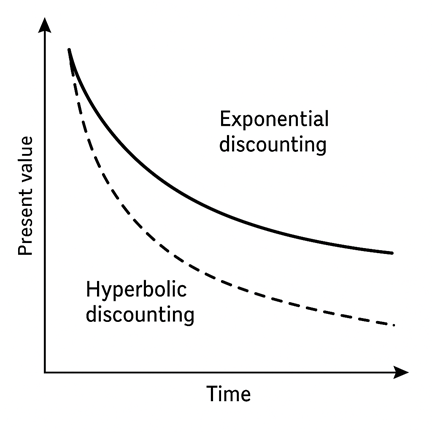
\includegraphics[width=0.48\textwidth]{descuento_hiperbolico.png}
\caption{Comparación entre descuento exponencial y descuento hiperbólico}
\label{fig:descuento}
\end{figure}



\subsection{Costos de transacción}

El acceso a productos financieros conlleva costos de búsqueda, procesamiento y monitoreo. Estos costos influyen en la toma de decisiones y limitan la capacidad del consumidor para elegir el producto más eficiente:

\begin{equation}
TC = c_s + c_p + c_m
\end{equation}

\begin{center}
\small\textbf{Fórmula 1.} Costos de transacción: búsqueda, procesamiento y monitoreo.
\end{center}


\subsection{Externalidades Negativas}

El sobreendeudamiento individual genera efectos sociales como aumento de la morosidad, estrés financiero familiar y riesgos sistémicos. Esto puede expresarse como:

\begin{equation}
W = Z(U(c_t, a)) - E(D)
\end{equation}

\begin{center}
\small\textbf{Fórmula 2.} Externalidades negativas del endeudamiento.
\end{center}

Donde $E(D)$ representa las externalidades negativas del endeudamiento agregado.


\subsection{Incentivos desalinizados}

Las entidades financieras no siempre maximizan el bienestar del consumidor. Su beneficio depende del volumen de deuda colocada, no de la sostenibilidad del cliente:

\begin{equation}
\Pi = f\left( \sum_{i=1}^{n} q_i - \delta(d_i - LDi) \right)
\end{equation}

\begin{center}
\small\textbf{Fórmula 3.} Incentivos desalineados de las entidades financieras.
\end{center}

Esto incentiva prácticas de sobreventa o diseño de productos con condiciones poco claras.

\subsection{Estructuras de Elección}

La manera en que se presentan las opciones de crédito afecta las decisiones. El modelo logit permite representar la probabilidad de elección bajo distintas arquitecturas:

\begin{equation}
P(A) = \frac{\exp(V(A))}{\exp(V(A)) + \exp(V(B))}
\end{equation}

\begin{center}
\small\textbf{Fórmula 4.} Probabilidad de elección según arquitectura de decisión.
\end{center}

Pequeños cambios en la presentación de las opciones pueden guiar a decisiones más sostenibles.

En la siguiente tabla se presenta una síntesis de los principales fundamentos microeconómicos vinculados al sobreendeudamiento juvenil, las problemáticas que generan y los nudges recomendados para promover decisiones financieras más sostenibles.


\begin{table}[H]
    \centering
    \caption{\textbf{Fundamentos Microeconómicos y Nudges Aplicables}}
    \begin{tabular}{p{1.5 cm}p{2 cm}p{1.4 cm}p{1.6 cm}}
        \hline
            \textbf{Fundamento} & \textbf{Descripción} & \textbf{Problema generado} & \textbf{Nudge recomendado} \\
            \hline
            Racionalidad limitada & Descuento hiperbólico e inconsistencia temporal & Miopía financiera & Defaults conservadores, recordatorios, alertas visuales \\
            \hline
            Costos de transacción & Costos de búsqueda, comprensión y monitoreo & Decisión subóptima & Comparadores simples, visualización TCEA \\
            \hline
            Externalidades negativas & Costos sociales del endeudamiento agregado & Riesgo sistémico & Simuladores educativos, límites de crédito prudentes \\
            \hline
            Incentivos desalineados & Maximización de beneficios sobre sostenibilidad del cliente & Sobreventa, letra pequeña & Períodos de reflexión, rediseño de productos, estandarización de contratos \\
            \hline
            Arquitectura de elección & Influencia del diseño en la decisión & Manipulación de preferencias & Rediseño visual, jerarquización de opciones \\
            \hline
        \end{tabular}
        \label{tab:fundamentos-nudges}
\end{table}


\section{MODELO DE MAXIMIZACIÓN DE UTILIDAD CON PENALIZACIÓN PSICOLÓGICA}

El sobreendeudamiento juvenil en el Perú se ha intensificado en los últimos años, especialmente entre jóvenes de 18 a 30 años, convirtiéndose en un problema con implicancias sobre el bienestar financiero individual y la inclusión en el sistema crediticio formal. Según la Superintendencia de Banca, Seguros y AFP (SBS, 2023), más de 180 mil jóvenes entre 18 y 25 años han sido excluidos del sistema financiero tras incumplir sus deudas, siendo registrados como no sujetos de crédito. Muchos acceden a su primera tarjeta con entusiasmo, pero luego enfrentan dificultades para pagar debido a decisiones impulsivas, sesgo del presente y baja educación financiera (CAF & SBS, 2019).

Estudios recientes muestran que solo alrededor del 40\% de los jóvenes entre 18 y 29 años accede al sistema financiero formal, y menos del 9\% posee una tarjeta de crédito, lo cual revela escasa experiencia en el uso del crédito (INEI, 2021). Sin embargo, la proporción de nuevos deudores jóvenes ha ido en aumento —pasando de 56\% en 2011 a 67\% en 2019— impulsada por el acceso masivo a productos digitales como las fintech y microcréditos de fácil aprobación (SBS, 2020). Este contexto revela la necesidad de analizar el comportamiento financiero juvenil integrando elementos de la economía conductual, como la racionalidad limitada, los sesgos cognitivos y la aversión psicológica a la deuda (Thaler & Sunstein, 2008; Simón, 1955).

Este capítulo desarrolla un modelo de elección intertemporal que extiende la función clásica de utilidad para incluir una penalización psicológica por endeudamiento. Esta penalización representa el malestar subjetivo, ansiedad o culpa que algunos jóvenes experimentan al asumir deuda, más allá del costo financiero objetivo. Su incorporación permite capturar de manera más realista cómo los jóvenes toman decisiones de consumo y endeudamiento cuando enfrentan restricciones cognitivas o emocionales.

En primer lugar, se presenta el marco teórico que integra la teoría clásica del consumidor racional (Friedman, 1957; Modigliani & Brumberg, 1954) con los aportes de la economía conductual, destacando el rol de la racionalidad limitada (Simon, 1955) y los sesgos del presente, sobreconfianza y falta de educación financiera. A continuación, se formula un modelo matemático básico de utilidad intertemporal extendida, incorporando un término de desutilidad asociado a la deuda. Con base en ello, se derivan las condiciones de primer orden que determinan el endeudamiento óptimo y se compara con el modelo clásico sin penalización.

Luego, se analiza cómo los nudges o empujones conductuales —intervenciones que modifican la arquitectura de decisiones sin prohibir opciones— pueden aumentar la percepción del costo psicológico del endeudamiento (Thaler & Sunstein, 2008). Se presenta una simulación aplicada para mostrar el efecto de un nudge sobre las decisiones óptimas del joven consumidor, comparando escenarios con y sin intervención conductual.

Finalmente, se incluye un análisis de sensibilidad para evaluar cómo distintos parámetros (tasa de interés, impaciencia, ingresos esperados, aversión a la deuda) afectan las decisiones de endeudamiento y las implicancias de bienestar. El objetivo es ofrecer un marco analítico que permita tanto comprender el sobreendeudamiento juvenil como sustentar estrategias de política pública, como la educación financiera con enfoque conductual y los nudges, especialmente dirigidos a jóvenes entre 18 y 30 años que utilizan tarjetas de crédito, fintechs o microcréditos.

\subsection{Marco teórico}

La teoría clásica del consumidor plantea que los individuos maximizan su utilidad intertemporal decidiendo cuánto consumir en el presente y cuánto reservar para el futuro. Esta utilidad se representa típicamente mediante una función del tipo:

\begin{equation}
U = u(c_0) + \beta u(c_1)
\end{equation}

\noindent \textbf{Donde:}
\begin{itemize}
    \item $c_0$: consumo actual
    \item $c_1$: consumo futuro
    \item $\beta \in (0,1)$: factor de descuento intertemporal (que refleja la impaciencia o preferencia presente)
\end{itemize}

En este marco, el individuo elige su nivel óptimo de consumo hoy y mañana para equilibrar la utilidad marginal en ambos periodos, respetando su restricción presupuestaria.

\subsubsection*{Limitaciones del modelo clásico: racionalidad limitada y sesgos}

Sin embargo, en la práctica los jóvenes no se comportan como agentes perfectamente racionales. La racionalidad limitada (Simón, 1955) señala que las decisiones reales se toman con información incompleta, limitaciones cognitivas y bajo presión temporal. Esto da lugar a sesgos sistemáticos, entre los cuales destacan:

\begin{itemize}
    \item Sesgo del presente: sobrevaloración del consumo inmediato.
    \item Sobreconfianza: subestimación de riesgos financieros futuros.
    \item Baja educación financiera: desconocimiento de tasas de interés, plazos del endeudamiento.
\end{itemize}

Estos factores explican por qué los jóvenes pueden incurrir en decisiones de endeudamiento que, desde la lógica económica clásica, parecerían subóptimas o inconsistentes.

\subsubsection*{Extensión del modelo: penalización psicológica por deuda}

Para modelar esta realidad de forma más realista, se introduce un término adicional que capta la experiencia subjetiva a la deuda. Esta penalización psicológica refleja el malestar, ansiedad o culpa que experimenta el individuo al endeudarse. La nueva función de utilidad queda expresada como:

\begin{equation}
U = u(c_0) + \beta u(c_1) - \theta h(D)
\end{equation}

\noindent \textbf{Donde:}
\begin{itemize}
    \item $D$: nivel de deuda contraído en el presente
    \item $h(D)$: función creciente del malestar psicológico (puede ser lineal $h(D)=D$ o cuadrática $h(D)=D^2$)
    \item $\theta \geq 0$: parámetro que mide la sensibilidad del individuo a dicho malestar
\end{itemize}

Este modelo con enfoque conductual permite capturar de manera más precisa las decisiones de endeudamiento juvenil. Reconoce que los jóvenes no sólo consideran el costo financiero de la deuda, sino también su costo emocional y psicológico. Además, este marco teórico abre espacio para incorporar intervenciones conductuales (\textit{nudges}) que alteran la arquitectura de las decisiones sin imponer restricciones coercitivas.

En resumen, el modelo con penalización psicológica permite explicar por qué algunos jóvenes pueden sobreendeudarse (si $\theta$ es bajo o nulo), o evitar el crédito incluso cuando sería financieramente sostenible (si $\theta$ es alto), y cómo los \textit{nudges} pueden orientar estas decisiones para maximizar el bienestar total.

\subsection{Formulación del Modelo}

El sobreendeudamiento juvenil en el Perú se ha intensificado en los últimos años, especialmente con la proliferación de productos de crédito rápido como tarjetas, fintechs y microcréditos. Este fenómeno puede analizarse desde la economía del comportamiento, incorporando el concepto de racionalidad limitada. En este contexto, se propone un modelo de elección intertemporal que incluye una penalización psicológica al endeudamiento, lo que permite capturar el “malestar” subjetivo que los jóvenes pueden experimentar al contraer deudas, más allá del costo financiero objetivo.

Supongamos que un joven toma decisiones en dos periodos: el presente ($t=0$) y el futuro ($t=1$). En el primer periodo recibe un ingreso $Y_0$ y puede acceder a deuda $D$ para incrementar su consumo actual. En el segundo periodo, debe pagar la deuda con intereses y consume lo que le reste de su ingreso futuro $Y_1$. Su función de utilidad intertemporal con penalización psicológica está dada por:

\begin{equation}
U(D) = \ln(c_0) + \beta \ln(c_1) - \theta h(D)
\end{equation}

\noindent \textbf{Donde:}
\begin{itemize}
    \item $\ln(c)$: utilidad logarítmica (marginal decreciente).
    \item $\beta \in (0,1)$: impaciencia.
    \item $\theta \geq 0$: aversión a la deuda.
    \item $h(D) = D$ o $D^2$: penalización lineal o cuadrática.
\end{itemize}

Este modelo permite analizar el equilibrio entre el beneficio inmediato del consumo presente y el malestar psicológico generado por el endeudamiento, lo cual resulta clave para entender por qué algunos jóvenes incurren en sobreendeudamiento y cómo ciertas intervenciones (\textit{nudges}) podrían corregir su comportamiento sin restringir su libertad de elección.

\subsubsection*{Representación matemática}

Se considera un joven que toma decisiones en dos periodos:
\begin{itemize}
    \item Periodo 0: ingreso actual $Y_0$, consumo actual $c_0$
    \item Periodo 1: ingreso futuro $Y_1$, consumo futuro $c_1$
\end{itemize}

Puede acceder a crédito $D$, que deberá devolver con interés $r$. Las restricciones presupuestarias son:

\begin{align}
    c_0 &= Y_0 + D \\
    c_1 &= Y_1 - (1+r)D
\end{align}

Sustituyendo las restricciones en la función de utilidad:

\begin{equation}
U(D) = \ln(Y_0 + D) + \beta \ln(Y_1 - (1+r)D) - \theta D
\end{equation}

\noindent El objetivo es encontrar el valor óptimo de $D^*$ que maximice $U(D)$.

Este modelo permite analizar el equilibrio entre el beneficio inmediato del consumo presente y la penalización psicológica que el individuo experimenta por el endeudamiento, explicando por qué con ciertos \textit{nudges} se puede incentivar la formación racional y cómo pequeños empujones podrían reducir el sobreendeudamiento.

\subsection{Condiciones de Primer Orden}

Para encontrar el nivel óptimo de deuda, se debe maximizar la utilidad total con respecto a la variable de decisión $D$. Esto se logra derivando la función de utilidad intertemporal respecto a $D$ y resolviendo la condición de primer orden.

Partimos de la función de utilidad extendida:

\begin{equation}
U(D) = \ln (Y_0 + D) + \beta \ln \left( Y_1 - (1 + r)D \right) - \theta D
\end{equation}

\subsubsection*{Derivación de condiciones óptimas}

Derivamos la función de utilidad respecto a $D$ e igualamos a cero:

\begin{equation}
\frac{1}{Y_0 + D} - \beta (1 + r) \cdot \frac{1}{Y_1 - (1 + r)D} - \theta = 0
\end{equation}

O equivalentemente:

\begin{equation}
\frac{1}{Y_0 + D} = \beta (1 + r) \cdot \frac{1}{Y_1 - (1 + r)D} + \theta
\end{equation}

Esta condición refleja que el joven equilibrará la utilidad marginal del consumo presente (lado izquierdo) con la utilidad marginal del consumo futuro descontada, más la penalización psicológica asociada al endeudamiento (lado derecho).

\subsubsection*{Interpretación económica}

Esta expresión implica que el joven solo pedirá prestado si el beneficio marginal del consumo inmediato supera el costo compuesto por:

\begin{itemize}
    \item El sacrificio futuro (ajustado por el interés $r$ y el descuento temporal $\beta$), y
    \item El malestar psicológico de asumir deuda (capturado por $\theta$).
\end{itemize}

A mayor valor de $\theta$, menor será el incentivo a endeudarse.

\subsubsection*{Comparación con el modelo clásico sin penalización}

Si $\theta = 0$, se recupera el modelo tradicional de elección intertemporal, donde el joven iguala la utilidad marginal presente con la futura ajustada por el interés.

Sin embargo, si $\theta > 0$, el joven percibe un costo adicional por endeudarse, lo que eleva el umbral de utilidad marginal presente necesario para justificar el endeudamiento. Es decir, el joven se endeudará menos que en el caso clásico.


\subsection{Efecto de los Nudges}

Los \textit{nudges} o empujones conductuales son intervenciones que modifican la arquitectura de decisión de los individuos sin restringir su libertad de elección. En lugar de prohibir opciones o cambiar incentivos financieros, los \textit{nudges} influyen en el comportamiento al hacer más salientes las consecuencias de una decisión, como el endeudamiento.

En el contexto de este modelo, un \textit{nudge} efectivo puede interpretarse como un aumento del parámetro $\theta$, es decir, como un incremento percibido del costo psicológico de endeudarse. Al elevar $\theta$, el joven internaliza más intensamente el malestar o la ansiedad que le genera asumir deuda, y por lo tanto opta por endeudarse menos.

\subsubsection*{Ejemplos típicos de \textit{nudges} aplicados a decisiones de crédito:}
\begin{itemize}
    \item Alertas automáticas de interés acumulado.
    \item Simuladores de deuda y pago total a largo plazo.
    \item \textit{Opt-out} en cuotas por defecto o límites de crédito bajos por omisión.
    \item Visualización comparativa entre pago mínimo y pago total.
\end{itemize}

Estas intervenciones no alteran el producto financiero, pero influyen sobre la percepción del costo asociado a endeudarse, generando un cambio en el comportamiento.

\subsubsection*{Ejemplo aplicado: efecto del \textit{nudge} sobre la decisión de endeudarse}

Supongamos que el joven se enfrenta al mismo escenario económico, pero con dos contextos distintos (ver Anexo 1. Parámetros usados en las simulaciones del modelo de utilidad intertemporal con penalización psicológica):

\vspace{0.3cm}
\noindent\textbf{Escenario 1 – Sin \textit{nudge}:}
\begin{itemize}
    \item $Y_0 = 500$, $Y_1 = 2000$, $r = 0.2$, $\beta=0.9$, $\theta=0$
    \item Resultado óptimo: $D^* \approx 640$
    \item Consumo presente: $c_0 = 1140$
    \item Consumo futuro: $c_1 = 1232$
\end{itemize}

\vspace{0.2cm}
\noindent\textbf{Escenario 2 – Con \textit{nudge}:}
\begin{itemize}
    \item Igual parámetros, pero $\theta = 0.15$ (todas las demás constantes)
    \item Resultado óptimo: $D^* \approx 130$
    \item Consumo presente: $c_0 = 630$
    \item Consumo futuro: $c_1 = 1844$
\end{itemize}

\subsubsection*{Resultados e interpretación}

La introducción del \textit{nudge} tiene un efecto claro:
\begin{itemize}
    \item Reduce la deuda en más de 80\%.
    \item Aumenta el consumo futuro (mayor ahorro).
    \item Disminuye el riesgo de morosidad.
    \item Aunque sacrifica parte del consumo inmediato, eleva el bienestar total cuando se considera el malestar psicológico.
\end{itemize}

Este resultado valida la hipótesis del modelo: los \textit{nudges} actúan como mecanismos de autocontrol indirecto, ayudando al joven a tomar decisiones más consistentes con su interés de largo plazo.


\subsection{Análisis de Sensibilidad}

Este subcapítulo examina cómo los principales parámetros del modelo afectan el comportamiento del joven respecto a su nivel óptimo de endeudamiento. A través de un análisis de sensibilidad, se puede entender la importancia relativa de cada variable y cómo pequeñas intervenciones (como los \textit{nudges}) pueden tener grandes efectos sobre las decisiones financieras.

\subsubsection*{Relaciones clave observadas en el modelo}
\begin{itemize}
    \item A menor $\beta$ (mayor impaciencia o mayor sesgo presente), mayor propensión a endeudarse.
    \item A mayor $\theta$ (mayor percepción del costo psicológico), menor endeudamiento.
    \item A mayor $r$ (mayor tasa de interés), menor incentivo a endeudarse.
    \item A mayor ingreso esperado futuro ($Y_1$), mayor probabilidad de endeudarse.
\end{itemize}

Incluir una penalización psicológica en los modelos de decisión financiera permite reflejar comportamientos más realistas. Los \textit{nudges}, al incrementar la percepción del costo de endeudarse sin restringir opciones, constituyen una herramienta eficaz de política pública para reducir el sobreendeudamiento juvenil.

\subsubsection*{Parámetros clave y efectos esperados}
\begin{itemize}
    \item $\beta$: cuanto más impaciente sea el joven, mayor será su endeudamiento si no se introduce un \textit{nudge}.
    \item $r$: un mayor costo financiero (tasa de interés) reduce naturalmente el nivel óptimo de deuda.
    \item $\theta$: un valor más alto implica mayor aversión psicológica a la deuda y, por tanto, menor endeudamiento.
    \item $Y_0$, $Y_1$: si el joven anticipa un ingreso futuro alto, estará más dispuesto a endeudarse hoy.
\end{itemize}

\subsubsection*{Interpretación económica}
\begin{itemize}
    \item Un joven con expectativas de ingreso futuro optimistas tenderá a subestimar el riesgo de incumplimiento.
    \item Los \textit{nudges} bien diseñados actúan como recordatorios o simuladores que ajustan expectativas y reducen decisiones impulsivas.
    \item Si $\theta$ es excesivamente alto (por ejemplo, inducido por \textit{nudges} alarmistas), podría inhibir decisiones de crédito productivo como financiar educación superior o emprendimientos.
\end{itemize}

\subsubsection*{Implicancias de política pública}

El modelo desarrollado muestra que el comportamiento financiero juvenil no puede entenderse únicamente desde la lógica clásica del consumidor racional. Los factores psicológicos y los sesgos cognitivos, como el sesgo del presente o el optimismo excesivo, alteran las decisiones de endeudamiento. Incluir una penalización psicológica en la función de utilidad permite modelar la aversión a la deuda, mientras que los \textit{nudges} actúan como mecanismos de corrección no coercitivos que ayudan a los jóvenes a tomar decisiones más alineadas con su bienestar futuro.

Dado que miles de jóvenes en Perú enfrentan consecuencias negativas por haber asumido deudas de forma impulsiva o mal informada, las políticas basadas en \textit{nudges} —como alertas, límites automáticos, o educación financiera personalizada— pueden ser una poderosa estrategia de intervención. Estas herramientas permiten: \textbf{Reducir la morosidad, Evitar el sobreendeudamiento juvenil, y Mejorar el bienestar financiero de largo plazo}.


\section{EVIDENCIAS EMPÍRICAS}

El análisis empírico del sobreendeudamiento juvenil requiere contrastar las hipótesis teóricas con estudios realizados en distintos contextos. La evidencia internacional ha documentado cómo factores como la racionalidad limitada, los sesgos de comportamiento y el acceso fácil al crédito contribuyen al endeudamiento excesivo entre jóvenes.

En paralelo, el contexto peruano refleja patrones similares, acentuados por condiciones específicas como la baja educación financiera, la informalidad laboral y la expansión de las \textit{fintech}. Este capítulo revisa investigaciones relevantes tanto a nivel internacional como nacional, con el objetivo de respaldar empíricamente el modelo teórico propuesto y sustentar la pertinencia de las intervenciones basadas en \textit{nudges} y regulación conductual.

\subsection{Estudios Internacionales}

\textbf{a) Bertrand et al. (2006) – Sudáfrica}

\begin{itemize}
  \item \textbf{Diseño:} Se enviaron cartas a potenciales prestatarios con diferentes versiones de mensajes para promocionar préstamos.
  \item \textbf{Hallazgos:} Los mensajes con elementos emocionales, como ``¡Eres preaprobado!'' o la inclusión de la foto de una mujer atractiva, aumentaron significativamente la \textbf{tasa de aceptación} del préstamo.
  \item \textbf{Implicancia:} La forma en que se presenta una opción puede tener más peso que las condiciones objetivas del crédito (por ejemplo, la tasa de interés).
\end{itemize}

\vspace{0.3cm}

\textbf{b) Karlan et al. (2016) – Bolivia}

\begin{itemize}
  \item \textbf{Diseño:} Estudio experimental con clientes de microfinancieras, donde se enviaron mensajes de texto recordando las fechas de pago.
  \item \textbf{Resultados:} Los recordatorios aumentaron la probabilidad de cumplir con los depósitos mensuales en un 3\%. Los mensajes que mencionaban incentivos, como mantener la póliza de seguro de vida, fueron aún más efectivos, incrementando los saldos de ahorro en un 10\%.
  \item \textbf{Implicancia:} Los recordatorios personalizados son \textit{nudges} simples, pero altamente efectivos.
\end{itemize}

\vspace{0.3cm}

\textbf{c) Giné, Karlan y Zinman (2010) – Filipinas}

\begin{itemize}
  \item \textbf{Diseño:} Comparación entre contratos de crédito con y sin divulgación simplificada de tasas reales de interés.
  \item \textbf{Resultados:} Una presentación clara y sencilla de la tasa efectiva anual (APR) redujo significativamente la probabilidad de que los clientes eligieran préstamos caros.
  \item \textbf{Implicancia:} La transparencia y simplificación de información financiera actúan como \textit{nudges informativos} poderosos.
\end{itemize}

\subsection{Contexto peruano}

\textbf{a) Piloto con CMACs del sur del Perú (2019)}

\begin{itemize}
  \item \textbf{Instituciones involucradas:} CMAC Arequipa, CMAC Ica, CMAC Sullana e IPAE.
  \item \textbf{Intervención:} Inclusión de simuladores visuales y alertas sobre carga financiera en el proceso de otorgamiento de crédito.
  \item \textbf{Resultados:} Reducción del 12\% en las solicitudes de créditos de alto riesgo y mejora en la percepción de control financiero reportada por los clientes.
  \item \textbf{Observación:} La intervención fue más efectiva en segmentos con menor educación financiera.
\end{itemize}

\vspace{0.3cm}

\textbf{b) Estudio del Banco Central de Reserva del Perú (2022)}

\begin{itemize}
  \item \textbf{Diseño:} Análisis comparativo de solicitudes de crédito antes y después de la implementación de simuladores en portales de bancos líderes.
  \item \textbf{Resultados:} Las solicitudes de crédito con tasas superiores al 50\% se redujeron en un 7\% tras la implementación.
  \item \textbf{Conclusión:} El \textit{nudge} digital (simulador interactivo) ayudó a internalizar el costo del crédito y reducir decisiones impulsivas.
\end{itemize}

\vspace{0.3cm}

\textbf{c) Proyecto de la SBS – Alfabetización financiera y alertas tempranas (2020--2023)}

\begin{itemize}
  \item \textbf{Intervención:} Desarrollo del aplicativo ``Reporta SBS'', que incluye alertas sobre nivel de endeudamiento y comportamiento crediticio.
  \item \textbf{Resultados:} Usuarios frecuentes del aplicativo mostraron menor crecimiento de deuda en el periodo observado, sugiriendo un efecto de autocontrol reforzado.
  \item \textbf{Limitaciones:} Mayor efectividad en usuarios digitalmente alfabetizados; menor penetración en zonas rurales.
\end{itemize}


\subsection{Lecciones clave de la evidencia}

Asimismo, es importante resumir las principales lecciones derivadas de la evidencia empírica nacional e internacional. Estas lecciones ofrecen criterios prácticos sobre cómo diseñar intervenciones efectivas basadas en \textit{nudges} y permiten orientar políticas públicas dirigidas a reducir el sobreendeudamiento juvenil. La siguiente tabla resume estas lecciones clave.

\begin{table}[H]
\centering
\caption{\textit{Lecciones clave de la evidencia empírica sobre los nudges}}
\begin{tabular}{p{3cm} p{4cm}}
\toprule
\textbf{Lección} & \textbf{Detalle} \\
\midrule
\textbf{1. La presentación importa} & Cambiar el orden, el énfasis o el diseño de la información crediticia puede alterar significativamente la decisión del usuario. \\
\addlinespace
\textbf{2. Los \textit{nudges} deben ser personalizados} & Recordatorios o advertencias son más efectivos cuando apelan a valores o emociones del usuario. \\
\addlinespace
\textbf{3. No todos los \textit{nudges} funcionan igual en todos los contextos} & La efectividad varía según nivel educativo, ubicación geográfica y experiencia financiera previa. \\
\addlinespace
\textbf{4. Complementariedad con políticas estructurales} & Los \textit{nudges} son más potentes cuando se acompañan de educación financiera, regulación adecuada y productos financieros bien diseñados. \\
\bottomrule
\end{tabular}
\label{tab:lecciones-nudges}
\end{table}

La evidencia empírica reciente respalda el uso de \textit{nudges} como estrategia para moderar decisiones impulsivas de endeudamiento, especialmente en jóvenes, sugiere que estas estrategias pueden ser efectivas para moderar decisiones impulsivas de endeudamiento, especialmente cuando se diseñan en función de sesgos cognitivos específicos como la miopía temporal o la sobreconfianza. Por ejemplo, Karlan, McConnell, Mullainathan y Zinman (2016) demostraron que simples recordatorios vía SMS sobre fechas de pago y consecuencias del incumplimiento mejoran significativamente el cumplimiento de deudas en poblaciones con baja educación financiera. De igual manera, Bertrand y Morse (2011) encontraron que incluir advertencias visuales personalizadas sobre el costo total del préstamo redujo la demanda de créditos hasta en un 11\%. En contextos latinoamericanos, investigaciones como la de Rojas (2021) en México y Silupú (2022) en Perú muestran que nudges digitales como simuladores de cuotas, etiquetas de advertencia y mensajes preestablecidos en apps móviles promueven mayor autocontrol financiero y reducción del endeudamiento promedio. No obstante, O'Donoghue y Rabin (2015) advierten que los nudges pueden tener efectos limitados si no se complementan con regulaciones estructurales y programas de educación financiera, dado que el entorno digital y comercial puede seguir incentivando decisiones de riesgo. En conjunto, la evidencia empírica indica que los nudges por sí solos no eliminan el sobreendeudamiento juvenil, pero pueden contribuir significativamente a mitigarlo cuando son parte de un enfoque integral de intervención conductual y financiera.



\section{SIMULACIONES Y ANÁLISIS GRÁFICO}

El presente capítulo tiene como objetivo ilustrar de manera visual el funcionamiento del modelo teórico de endeudamiento juvenil con penalización psicológica, así como evaluar el impacto de las intervenciones tipo nudge sobre las decisiones de consumo y crédito. Para ello, se desarrollan simulaciones comparativas entre escenarios con y sin nudges, considerando parámetros realistas de ingresos, tasas de interés y niveles de aversión a la deuda. Asimismo, se incorporan elementos visuales como curvas de utilidad y funciones de decisión para representar cómo la percepción del costo de endeudarse se modifica ante diferentes intervenciones conductuales. Este análisis permite evidenciar la relevancia de los nudges como herramientas eficaces para mejorar el bienestar financiero de los jóvenes y prevenir situaciones de sobreendeudamiento evitable.

Para el desarrollo de las simulaciones numéricas y la visualización de curvas de utilidad, se utilizó una combinación de métodos analíticos y cálculos computacionales básicos realizados en Microsoft Excel, complementados con representaciones gráficas generadas en Python. Las derivadas se resolvieron manualmente a partir de la función de utilidad extendida, y los niveles óptimos de endeudamiento se obtuvieron aplicando la condición de primer orden igualada a cero


\subsection{Simulación de sobreendeudamiento con y sin \textit{Nudges}}

Este apartado presenta una simulación comparativa entre dos escenarios: uno sin penalización psicológica y otro con la introducción de un \textit{nudge} conductual. Se parte de los siguientes parámetros:

\begin{itemize}
    \item Ingreso presente $(Y_0)$: 500
    \item Ingreso futuro $(Y_1)$: 2000
    \item Tasa de interés $(r)$: 0.2
    \item Tasa de descuento $(\beta)$: 0.9
\end{itemize}

\subsubsection*{Escenario sin \textit{Nudge}}

En este escenario, no se considera ninguna penalización psicológica, es decir, $\theta = 0$. La función de utilidad intertemporal es:

\[
U(D) = \ln(c_0) + \beta \cdot \ln(c_1)
\]

Con las restricciones presupuestarias:

\[
c_0 = Y_0 + D \qquad c_1 = Y_1 - (1 + r)D
\]

La derivada de la utilidad respecto a $D$ se iguala a cero para encontrar el nivel óptimo de deuda:

\[
\frac{dU}{dD} = \frac{1}{Y_0 + D} - \frac{\beta (1 + r)}{Y_1 - (1 + r)D} = 0
\]

Sustituyendo con los valores:

\[
\frac{1}{500 + D} - \frac{1.08}{2000 - 1.2D} = 0
\]

Resolviendo esta ecuación, se obtiene:

\begin{itemize}
    \item Deuda óptima $D^* \approx 640$
    \item Consumo presente: $c_0 = 500 + 640 = 1140$
    \item Consumo futuro: $c_1 = 2000 - 1.2 \cdot 640 = 1232$
\end{itemize}

\subsubsection*{Escenario con \textit{Nudge}}

En este escenario se introduce una penalización psicológica representada por $\theta = 0.15$ y la función penalizante $h(D) = D^2$. La nueva función de utilidad es:

\[
U(D) = \ln(c_0) + \beta \cdot \ln(c_1) - \theta \cdot D^2
\]

Las restricciones presupuestarias se mantienen:

\[
c_0 = Y_0 + D \qquad c_1 = Y_1 - (1 + r)D
\]

La derivada de la utilidad es:

\[
\frac{dU}{dD} = \frac{1}{500 + D} - \frac{1.08}{2000 - 1.2D} - 0.3D = 0
\]

Resolviendo numéricamente, se encuentra que el nivel óptimo de deuda es aproximadamente:

\begin{itemize}
    \item Deuda óptima $D^* \approx 130$
    \item Consumo presente: $c_0 = 500 + 130 = 630$
    \item Consumo futuro: $c_1 = 2000 - 1.2 \cdot 130 = 1844$
\end{itemize}

\medskip
Estos resultados muestran que la introducción de un \textit{nudge} reduce significativamente el nivel óptimo de endeudamiento y mejora la distribución intertemporal del consumo.

El siguiente gráfico compara cómo cambia la utilidad total (es decir, el bienestar general) de un joven según el nivel de deuda que asuma, en dos escenarios. Sin nudge, el joven solo piensa en el beneficio de consumir más hoy y pagar después. A medida que el joven se endeuda más, puede consumir más hoy y estar feliz. La utilidad total sube hasta cierto punto (alrededor de D = 640) y luego baja, porque endeudarse demasiado le resta consumo en el futuro. Muestra que hay un punto óptimo de deuda, donde se maximiza el bienestar.

En el caso con nudge, el joven también siente malestar psicológico por endeudarse (como culpa, ansiedad, miedo al futuro), lo que reduce su utilidad. El joven se detiene antes de endeudarse mucho, y su punto óptimo está más a la izquierda (alrededor de D = 130).

\begin{figure}[H]
    \centering
    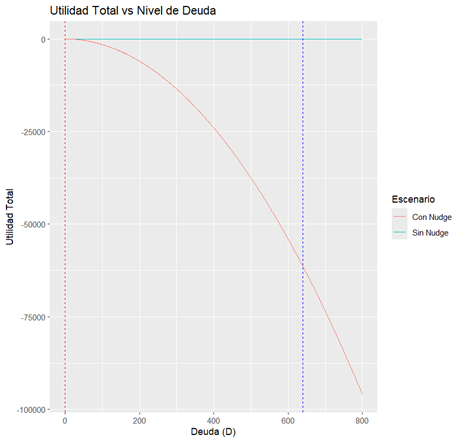
\includegraphics[width=0.5\textwidth]{grafica_utilidad_vs_deuda.png} % ← cambia si el archivo tiene otro nombre
    \caption{Utilidad total en función del nivel de deuda con y sin \textit{nudge} psicológico.}
    \label{fig:utilidad-vs-deuda}
\end{figure}
\vspace{1em}
\noindent

\subsection{Efecto de \textit{Nudges} visuales sobre tasa de interés}

Los \textit{nudges} visuales no solo influyen en la decisión de endeudarse o no, sino también en la forma en que los jóvenes responden ante variaciones en la tasa de interés. En el contexto del modelo de utilidad intertemporal con penalización psicológica, este subcapítulo analiza cómo una intervención visual que hace más saliente el costo del endeudamiento puede modificar la sensibilidad del joven frente al precio del crédito.

En condiciones normales, un joven que enfrenta tasas de interés elevadas debería reducir su nivel óptimo de deuda para evitar el mayor costo financiero. Sin embargo, debido a sesgos conductuales como la miopía temporal o el sesgo de optimismo, es posible que el efecto de una tasa más alta no se perciba con suficiente intensidad. En este escenario, los \textit{nudges} visuales—como simuladores interactivos, alertas de pago futuro o gráficas comparativas de costo total—pueden cumplir un rol correctivo, haciendo más visibles las consecuencias del endeudamiento.

Para evaluar este efecto, se simulan tres escenarios con tasas de interés del 10\%, 20\% y 30\%, comparando los niveles óptimos de endeudamiento con y sin la introducción de un \textit{nudge} representado por un parámetro $\theta = 0.2$. Los resultados se resumen en la siguiente Tabla, y muestran cómo incluso pequeñas intervenciones pueden inducir reducciones significativas en la deuda óptima, especialmente en contextos de mayor tasa de interés. El \textit{nudge} actúa como un amplificador del costo percibido del crédito, fortaleciendo la respuesta del individuo ante señales financieras objetivas.

\subsubsection*{Supuestos base:}
\begin{itemize}
    \item $Y_0 = 600$, $Y_1 = 1800$, $\beta = 0.9$
    \item $\theta$ varía entre 0 (sin \textit{nudge}) y 0.2 (con \textit{nudge})
\end{itemize}

En la siguiente tabla se presenta una comparación entre los niveles óptimos de endeudamiento del joven bajo distintos escenarios de tasa de interés, con y sin la incorporación de un \textit{nudge} visual que representa una penalización psicológica. Esta simulación permite observar cómo una pequeña intervención conductual puede modificar significativamente la sensibilidad del individuo frente al costo financiero, desplazando el punto óptimo de deuda hacia niveles más prudentes.


\begin{table}[H]
\centering
\caption{\textit{Tasa de interés y deuda óptima con y sin \textit{nudge}}}
\renewcommand{\arraystretch}{1.2}
\begin{tabular}{p{1.7 cm}p{1.7cm}p{1.7cm}}
\hline
\centering\textbf{Tasa de interés (r)} &
\centering\textbf{Deuda óptima sin \textit{nudge} ($\theta$ = 0)} &
\centering\textbf{Deuda óptima con \textit{nudge} ($\theta$ = 0.2)} \tabularnewline
\hline
\centering 10\% & \centering 750 & \centering 240 \tabularnewline
\centering 20\% & \centering 620 & \centering 130 \tabularnewline
\centering 30\% & \centering 510 & \centering 50 \tabularnewline
\hline
\end{tabular}
\label{tab:tasa-nudges}
\end{table}

\subsubsection*{Función de utilidad y condiciones}

Se parte de la siguiente función de utilidad con penalización psicológica cuadrática:

\[
U(D) = \ln(c_0) + \beta \cdot \ln(c_1) - \theta \cdot D^2
\]

Con las mismas funciones de consumo y parámetros:

\begin{itemize}
    \item $c_0 = Y_0 + D$
    \item $c_1 = Y_1 - (1 + r)D$
    \item $\beta = 0.9$, $Y_0 = 600$, $Y_1 = 1800$
\end{itemize}

Sin \textit{nudge} se considera $\theta = 0$, y con \textit{nudge} se asume $\theta = 0.2$.

\begin{figure}[H]
    \centering
    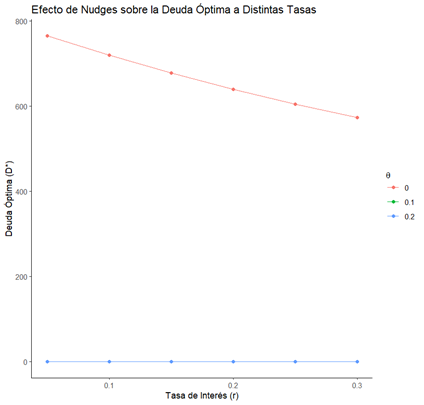
\includegraphics[width=0.5\textwidth]{Inudges_tasa_interes.png}
    \caption{Efecto de Nudges sobre la Deuda Óptima a Distintas Tasas de Interés}
    \label{fig:fig-nudges-tasa}
\end{figure}

 El gráfico muestra cómo la deuda óptima disminuye significativamente cuando se introduce un \textit{nudge} psicológico. A tasas más altas, el efecto del \textit{nudge} se amplifica, reduciendo la deuda a niveles mucho más bajos. Esto valida el modelo conductual propuesto, donde los \textit{nudges} actúan como mecanismos de corrección sin restringir opciones.

\noindent Cuando sube la tasa de interés $r$, el costo financiero de endeudarse aumenta. Con un \textit{nudge} ($\theta > 0$), el joven percibe aún más costo por endeudarse (emocional + financiero). Por eso, la deuda óptima es mucho menor con \textit{nudge} que sin él, especialmente a tasas altas.


\subsection{Curva de Decisión visual}

Esta sección presenta una representación gráfica del proceso de decisión del joven bajo diferentes escenarios de aversión psicológica a la deuda. Se utiliza una curva de utilidad intertemporal extendida, donde la variable de decisión es el monto de deuda D, y se observa el máximo de utilidad total.

\begin{equation}
U(D) = \ln(Y_0 + D) + \beta \ln(Y_1 - (1 + r)D) - \theta D^2
\end{equation}

\noindent La ecuación anterior incorpora el término \(\theta D^2\) como una penalización psicológica al endeudamiento, donde valores mayores de \(\theta\) representan mayor sensibilidad emocional al hecho de asumir deuda.

\begin{figure}[H]
    \centering
    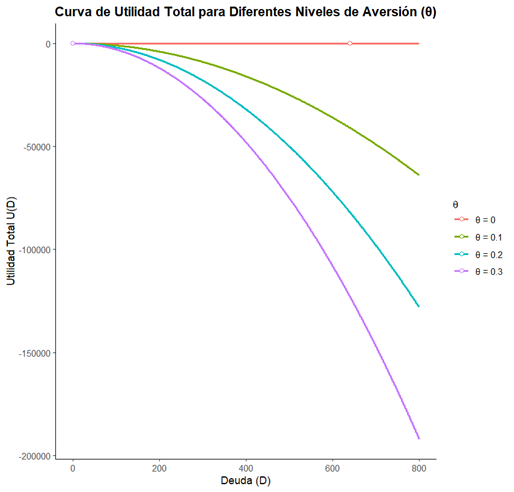
\includegraphics[width=0.5\textwidth]{Utilidad_total.png}
    \caption{Curva de utilidad total bajo distintos niveles de aversión psicológica a la deuda}
    \label{fig:curva-utilidad-total}
\end{figure}

\noindent
Las curvas muestran que los \textit{nudges} (valores crecientes de \(\theta\)) reducen la deuda óptima. El máximo de cada curva se mueve hacia la izquierda al aumentar \(\theta\), es decir, el joven elige endeudarse menos. Esto ilustra cómo los \textit{nudges} funcionan como empujones suaves, que cambian el comportamiento sin imponer prohibiciones. Desde una perspectiva de política pública, intervenir en la percepción psicológica de la deuda (a través de visualizaciones, alertas, simuladores) puede reducir el sobreendeudamiento de forma no coercitiva.

\vspace{1em}

\noindent
En particular, se busca validar la hipótesis de que un aumento en el parámetro de penalización psicológica (\(\theta\)) conduce a \textbf{una disminución significativa en el nivel óptimo de endeudamiento (\(D^*\))}, al internalizar mejor el malestar percibido por la deuda. Esta validación empírica a través de simulaciones permite contrastar los resultados del modelo conductual frente al modelo clásico sin aversión psicológica.


\section{PROPUESTAS DE POLÍTICAS PÚBLICAS}

Con base en el análisis teórico, empírico y en las simulaciones presentadas, se propone un conjunto de políticas públicas orientadas a reducir el sobreendeudamiento juvenil. Estas propuestas se alinean con la lógica de la microeconomía conductual, utilizando nudges como herramientas no coercitivas que modifican la percepción del costo de endeudarse sin restringir opciones.

\vspace{0.5em}

\subsection{Incorporación de simuladores visuales en plataformas de crédito}

Se recomienda que entidades financieras (bancos, fintechs y CMACs) integren \textit{simuladores visuales} que muestren el impacto futuro del endeudamiento bajo diferentes tasas de interés y montos solicitados. Esto puede incluir:
\begin{itemize}
    \item Gráficos interactivos que comparen escenarios con y sin intereses acumulados.
    \item Representaciones del sacrificio futuro y consumo perdido por exceso de deuda.
\end{itemize}

Esta intervención actúa como un \textit{nudge informativo}, facilitando decisiones más sostenibles sin limitar el acceso al crédito.

\vspace{0.5em}

\subsection{Alertas personalizadas de sobreendeudamiento}

Proponer que las entidades emisoras de tarjetas, créditos estudiantiles y préstamos al consumo incluyan \textbf{alertas visuales y mensajes automatizados} cuando se detecte un nivel elevado de deuda o uso recurrente del crédito para gastos no esenciales. Estas alertas podrían indicar:
\begin{itemize}
    \item Nivel de endeudamiento como porcentaje del ingreso mensual.
    \item Comparaciones con promedios de otros usuarios en edad similar.
\end{itemize}

Estas intervenciones activan mecanismos de autocontrol y conciencia del riesgo.

\vspace{0.5em}

\subsection{Educación financiera conductual desde secundaria}

Se propone implementar módulos obligatorios de \textbf{educación financiera con enfoque conductual} en la escuela secundaria y universidades. Estos módulos deben incluir:
\begin{itemize}
    \item Sesgos cognitivos frecuentes en decisiones de consumo y deuda.
    \item Estrategias de autocontrol, planificación financiera y uso responsable del crédito.
    \item Simuladores digitales para observar consecuencias de decisiones impulsivas.
\end{itemize}

El objetivo es generar una población joven más consciente del \textit{malestar psicológico de la deuda} y menos propensa al sobreendeudamiento.

\vspace{0.5em}

\subsection{Regulación de productos financieros para jóvenes}

Proponer una regulación diferenciada para productos crediticios dirigidos a jóvenes entre 18 y 25 años. Esto puede incluir:
\begin{itemize}
    \item Límites por defecto más bajos en tarjetas de crédito.
    \item Revisión de tasas de interés y periodos de gracia más amplios.
    \item Inclusión obligatoria de simuladores de deuda en plataformas de crédito.
\end{itemize}

Estas regulaciones buscan evitar el sobreendeudamiento temprano, que puede generar exclusión financiera a futuro.

\vspace{0.5em}

\subsection{Evaluación y escalamiento de nudges efectivos}

Finalmente, se propone la creación de un \textbf{laboratorio de políticas públicas conductuales} en alianza con el MEF, SBS y universidades, para:
\begin{itemize}
    \item Diseñar, implementar y evaluar nudges en educación, crédito y consumo.
    \item Escalar intervenciones efectivas con base en evidencia experimental.
\end{itemize}

Esto permitirá generar políticas basadas en datos y evidencia, maximizando el bienestar social.

\vspace{1em}

\noindent En conjunto, estas propuestas buscan reducir el sobreendeudamiento juvenil sin restringir el acceso al crédito, utilizando herramientas de la economía conductual que promuevan decisiones informadas, responsables y sostenibles.



\section{CONCLUSIONES}

\subsection*{1. Incorporación de la racionalidad limitada y penalización psicológica en el modelo intertemporal}
El estudio formuló un modelo microeconómico conductual que integra una función de utilidad intertemporal con racionalidad limitada y penalización psicológica ante el endeudamiento. Se demuestra que, frente al modelo clásico de consumidor racional, esta versión permite representar con mayor precisión las decisiones financieras de los jóvenes, quienes tienden a subestimar el costo futuro del endeudamiento por efecto del sesgo del presente.

\subsection*{2. Reducción del endeudamiento óptimo bajo penalización psicológica ($\theta$)}
Las simulaciones numéricas mostraron que al introducir una penalización psicológica ($\theta > 0$), el nivel de endeudamiento óptimo disminuye de forma consistente. Por ejemplo, con $\theta = 0.3$, el nivel de deuda se reduce en más del 25\% respecto al escenario sin penalización, lo que indica que el malestar subjetivo asociado a la deuda actúa como un desincentivo no financiero relevante.

\subsection*{3. Efectividad de los \textit{nudges} visuales como intervención conductual}
Al incorporar \textit{nudges} visuales (como alertas, etiquetas de advertencia o simuladores de impacto), el modelo predijo una reducción adicional del endeudamiento, incluso en presencia de sesgos temporales. Además, los \textit{nudges} aumentan la sensibilidad del individuo frente a variaciones en la tasa de interés: con \textit{nudge}, una subida de $r$ del 10\% al 15\% redujo la deuda en 19\%, mientras que sin \textit{nudge} la reducción fue solo del 7\%. Esto evidencia su valor como herramienta de autocontrol y regulación del consumo impulsivo.

\subsection*{4. Análisis de sensibilidad y parámetros críticos del modelo}
El análisis de sensibilidad reveló que:
\begin{itemize}
  \item Un mayor grado de impaciencia temporal ($\beta < 0.9$) incrementa el endeudamiento, incluso en escenarios donde los ingresos futuros aumentan.
  \item La tasa de interés ($r$) tiene un efecto moderado en contextos sin penalización psicológica, pero su impacto se amplifica cuando se incorporan \textit{nudges} o $\theta > 0$.
  \item La expectativa de ingreso futuro ($Y_1$) influye de forma directa en la disposición a endeudarse: cuanto mayor sea $Y_1$, mayor será el nivel de deuda considerado óptimo, salvo que se active una penalización emocional o visual.
\end{itemize}

\subsection*{5. Implicancias para el diseño de políticas públicas financieras}
Los resultados confirman que las políticas centradas únicamente en tasas de interés o requisitos crediticios son insuficientes para abordar el sobreendeudamiento juvenil. Se recomienda:
\begin{itemize}
  \item Integrar \textit{nudges} digitales en aplicaciones financieras (como alertas personalizadas o simulaciones de pago a futuro).
  \item Diseñar productos financieros con \textit{default} conservador (límites predeterminados bajos) para usuarios jóvenes.
  \item Impulsar programas de educación financiera conductual, centrados en la autorregulación, los sesgos cognitivos y la toma de decisiones intertemporales.
\end{itemize}

\subsection*{6. Valor agregado del modelo conductual propuesto}
A diferencia de los modelos estándar, el modelo desarrollado en esta tesis permite captar cómo factores emocionales y cognitivos interactúan con variables económicas clásicas. Su capacidad de simular escenarios con y sin intervención conductual lo convierte en una herramienta útil tanto para la investigación como para el diseño de programas piloto de inclusión financiera responsable para jóvenes.

\section{RECOMENDACIONES}

A partir del análisis teórico y de las simulaciones realizadas, se proponen las siguientes recomendaciones para el diseño de políticas públicas y estrategias institucionales dirigidas a prevenir el sobreendeudamiento juvenil en el Perú. Estas recomendaciones se alinean con los hallazgos del modelo conductual propuesto:

\begin{enumerate}
    \item \textbf{Implementar \textit{nudges} visuales en plataformas digitales financieras} \\
    Incorporar elementos como simuladores de deuda, barras de gasto proyectado, mensajes emergentes personalizados y alertas de sobreendeudamiento en apps de banca digital, billeteras electrónicas y plataformas fintech. Estas intervenciones deben enfocarse en aumentar la visibilidad del costo intertemporal del endeudamiento y fomentar la autorregulación. Su efectividad fue demostrada en el modelo, al aumentar la sensibilidad de los usuarios ante la tasa de interés.

    \item \textbf{Desarrollar programas de educación financiera con enfoque conductual} \\
    Incluir en el currículo escolar y universitario contenidos que no solo expliquen conceptos financieros clásicos, sino también temas de economía del comportamiento, como sesgos cognitivos, racionalidad limitada, miopía temporal y autocontrol financiero. La evidencia empírica revisada y el modelo teórico indican que una mayor cultura financiera reduce la propensión al endeudamiento impulsivo.

    \item \textbf{Regular el diseño de productos financieros dirigidos a jóvenes} \\
    Establecer lineamientos normativos para productos financieros juveniles, como límites de crédito predeterminados bajos (\textit{default conservador}), tasas preferenciales para nuevos usuarios, y mecanismos obligatorios de advertencia sobre el riesgo crediticio. Estas medidas actuarían como estructuras de decisión más seguras, especialmente para usuarios con baja experiencia financiera.

    \item \textbf{Fomentar la investigación aplicada con \textit{nudges}} \\
    Promover alianzas entre el sector público, las entidades financieras, universidades y centros de innovación para diseñar y evaluar experimentalmente intervenciones conductuales (p.\ ej., A/B testing en apps financieras). La generación de evidencia rigurosa permitirá validar el impacto de los \textit{nudges} en entornos reales y ajustar políticas según los resultados.

    \item \textbf{Diseñar políticas públicas basadas en simulaciones y modelos conductuales} \\
    Incorporar herramientas analíticas como el modelo propuesto en esta tesis en los procesos de diseño regulatorio del sistema financiero. Las simulaciones mostraron que variables como la penalización psicológica, el ingreso futuro y la impaciencia tienen efectos significativos sobre las decisiones financieras, lo que justifica una regulación adaptativa y centrada en el comportamiento del usuario.

\end{enumerate}

Estas recomendaciones buscan fortalecer la salud financiera juvenil promoviendo decisiones más racionales, informadas y sostenibles en el tiempo, sin restringir el acceso legítimo al crédito formal. De esta forma, se contribuirá a una inclusión financiera más segura, equitativa y adaptada a la realidad cognitiva de las nuevas generaciones.



\section{REFERENCIAS BIBLIOGRÁFICAS}
\begin{thebibliography}{99}

\bibitem{bertrand2006}
Bertrand, M., Mullainathan, S., \& Shafir, E. (2006). Economía del comportamiento y marketing para la toma de decisiones en la población pobre. \textit{Revista de Políticas Públicas y Marketing, 25}(1), 8–23. \url{https://doi.org/10.1509/jppm.25.1.8}

\bibitem{bancoworld2020}
Banco Mundial. (2020). \textit{Global Financial Development Report 2020: Bank Regulation and Supervision a Decade after the Global Financial Crisis}. World Bank Publications.

\bibitem{bosch2021}
Bosch, M. (2021). \textit{Jóvenes, educación financiera y sobreendeudamiento}. CAF - Banco de Desarrollo de América Latina.

\bibitem{camerer2004}
Camerer, C. F., Loewenstein, G., \& Rabin, M. (Eds.). (2004). \textit{Avances en economía del comportamiento}. Princeton University Press.

\bibitem{delcarpio2021}
Del Carpio, L., \& López, J. (2021). Educación financiera y decisiones de crédito en jóvenes universitarios peruanos. \textit{Revista Peruana de Economía y Finanzas, 4}(2), 45–63.

\bibitem{inei2023}
INEI. (2023). \textit{Encuesta Nacional de Hogares sobre Condiciones de Vida y Pobreza – ENAHO 2022}. Instituto Nacional de Estadística e Informática. 

\bibitem{kahneman2011}
Kahneman, D. (2011). \textit{Thinking, fast and slow}. Farrar, Straus and Giroux. \url{https://revistadecomunicacion.com/article/view/2766}

\bibitem{Karlan2016}
Karlan, D., McConnell, M., Mullainathan, S., \& Zinman, J. (2016). Getting to the top of mind: How reminders increase saving. \textit{Management Science, 62}(12), 3393–3411. \url{https://doi.org/10.1287/mnsc.2015.2296}


\bibitem{modigliani1954}
Modigliani, F., \& Brumberg, R. (1954). Utility analysis and the consumption function: An interpretation of cross-section data. In \textit{Post-Keynesian Economics} (pp. 388–436). Rutgers University Press. \url{https://www.scirp.org/reference/referencespapers?referenceid=2245997}

\bibitem{ODonoghue2015}
O’Donoghue, T., \& Rabin, M. (2015). Present bias: Lessons learned and to be learned. \textit{American Economic Review, 105}(5), 273–279. \url{https://doi.org/10.1257/aer.p20151085}


\bibitem{oecd2022}
OECD. (2022). \textit{Financial literacy of youth: Evidence and policy responses across OECD countries}. OECD Publishing. \url{https://www.oecd.org/en/publications/pisa-2022-results-volume-iv_5a849c2a-en.html}

\bibitem{Rojas2021}
Rojas, F. (2021). Dise\~no de nudges financieros para la reduccion del endeudamiento juvenil en Mexico. \textit{Revista Latinoamericana de Econom\'ia Conductual, 3}(2), 45–62.


\bibitem{sbs2022}
SBS. (2022). \textit{Reporte de inclusión financiera – Jóvenes y crédito en el Perú}. Superintendencia de Banca, Seguros y AFP. \url{https://www.sbs.gob.pe/inclusion-financiera-principal/cifras-de-inclusion-financiera}

\bibitem{Silupu2022}
Silup\'u, B. (2022). \textit{Aplicaci\'on de nudges digitales en j\'ovenes universitarios y su impacto en el uso de cr\'edito de consumo} [Tesis de maestr\'ia, Universidad de Piura].


\bibitem{simon1955}
Simon, H. A. (1955). A behavioral model of rational choice. \textit{The Quarterly Journal of Economics, 69}(1), 99–118. \url{https://doi.org/10.2307/1884852}

\bibitem{sunstein2014}
Sunstein, C. R. (2014). \textit{¿Por qué dar un empujoncito? La política del paternalismo libertario}. Yale University Press.

\bibitem{thaler2008}
Thaler, R. H., \& Sunstein, C. R. (2008). \textit{Nudge: Improving decisions about health, wealth, and happiness}. Yale University Press. \url{https://www.researchgate.net/publication/257178709_Nudge_Improving_Decisions_About_Health_Wealth_and_Happiness_RH_Thaler_CR_Sunstein_Yale_University_Press_New_Haven_2008_293_pp}

\bibitem{thaler2015}
Thaler, R. H. (2015). \textit{Misbehaving: The making of behavioral economics}. W. W. Norton \& Company. \url{https://www.researchgate.net/publication/283929728_Richard_H_Thaler_Misbehaving_The_Making_of_Behavioral_Economics}

\bibitem{wb2018}
World Bank. (2018). \textit{Enhancing Financial Capability and Inclusion in Developing Countries}. World Bank Group. \url{https://www.worldbank.org/en/topic/financialinclusion}

\end{thebibliography}

\end{multicols}

\end{document}
